\documentclass[tikz, convert={outfile=fisdat.svg}]{standalone}
\usepackage{amsmath}
\usetikzlibrary{arrows, fit, shapes}
\begin{document}
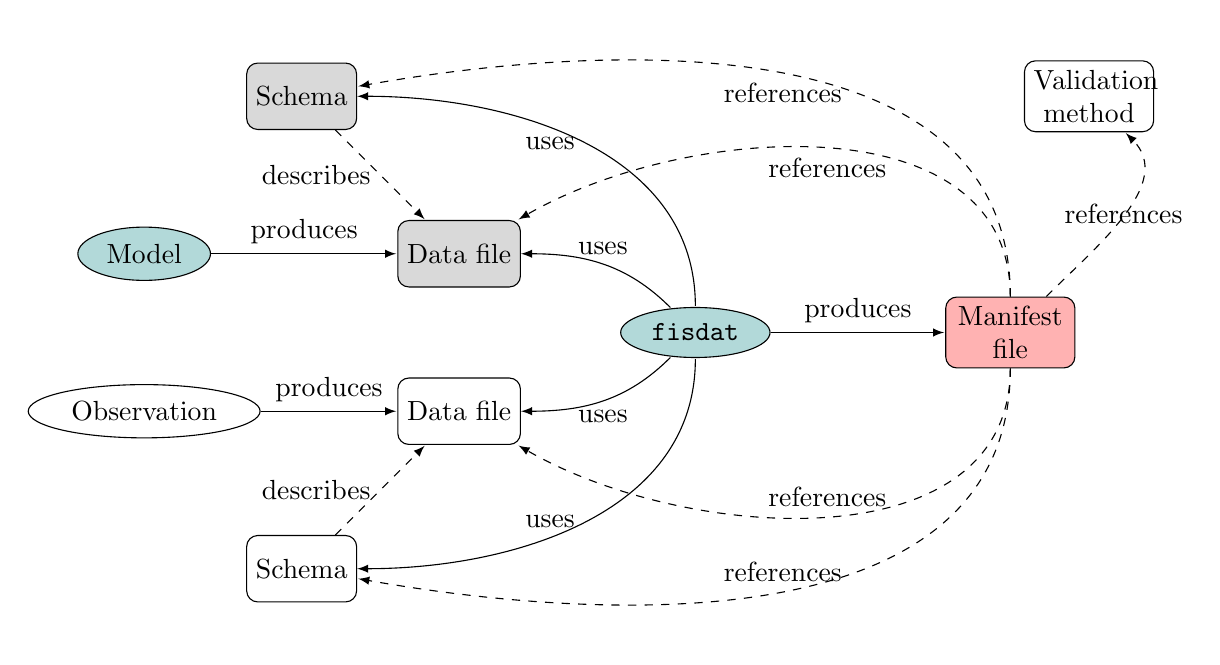
\begin{tikzpicture}[
    scale=1,
    box/.style={draw,ellipse},
    data/.style={draw,rounded corners,minimum height=2\baselineskip},
    refd/.style={draw,dashed,-latex,shorten >=0.4pt},
    used/.style={draw,latex-,shorten >=0.4pt},
    proc/.style={draw,-latex,shorten >=0.4pt},
    transform shape]
  \node[box,fill=teal!30] (densmodel) at (-4,1) { Model };
  \node[data,fill=gray!30] at (0,1) (densout) { Data file };
  \draw[proc] (densmodel) -- node[above] { produces } (densout);
  \node[data,fill=gray!30] (densschm) at (-2,3) { Schema };
  \draw[refd] (densschm) -- node[left] { describes } (densout);
  \node[box] (obs) at (-4,-1) { Observation };
  \node[data] at (0,-1) (obsout) { Data file };
  \draw[proc] (obs) -- node[above] { produces } (obsout);
  \node[data] (obsschm) at (-2,-3) { Schema };
  \draw[refd] (obsschm) -- node[left] { describes } (obsout);
  \node[box,fill=teal!30] (fisdat) at (3,0) { \texttt{fisdat} };
  \path[used] (densschm) edge[out=0,in=90] node[left] { uses } (fisdat);
  \path[used] (densout) edge[out=0,in=135] node[above] { uses } (fisdat);
  \path[used] (obsschm) edge[out=0,in=270] node[left] { uses } (fisdat);
  \path[used] (obsout) edge[out=0,in=225] node[below] { uses } (fisdat);
  \node[data,fill=red!30] (manif) at (7,0) { \parbox{4em}{\centering Manifest\\file} };
  \draw[proc] (fisdat) -- node[above] { produces } (manif);
  \path[refd] (manif) edge[out=90,in=10] node[below] { references } (densschm);
  \path[refd] (manif) edge[out=90,in=30] node[below] { references } (densout);
  \path[refd] (manif) edge[out=-90,in=-10] node[above] { references } (obsschm);
  \path[refd] (manif) edge[out=-90,in=-30] node[above] { references } (obsout);
  \node[data] (job) at (8,3) { \parbox{4em}{\centering Validation\\method} };
  \path[refd] (manif) edge[out=45,in=315] node { references } (job);
\end{tikzpicture}
\end{document}




